\documentclass[table]{beamer}
%%\documentclass[handout]{beamer}

\mode<presentation>
{
  \definecolor{navitialight}{RGB}{126,186,200}
  \definecolor{navitiadark}{RGB}{76,102,114}

  \useoutertheme[subsection=false]{miniframes}
  %%\useoutertheme[footline=authortitle]{miniframes}
  \usecolortheme[named=navitiadark]{structure}
  %%\usecolortheme{dolphin}
  \usecolortheme{orchid}
  \useinnertheme{circles}
  \setbeamerfont{block title}{size=\normalsize}
  \setbeamercovered{transparent}

  %%% le foot pour avoir la numérotation des slides %%%
  \setbeamertemplate{footline}{%
    \leavevmode%
    \hbox{%
      \begin{beamercolorbox}[wd=.5\paperwidth,ht=2.5ex,dp=1.125ex,
        leftskip=.3cm plus1fill,rightskip=.3cm]{author in head/foot}%
        \usebeamerfont{title in head/foot}\insertshorttitle
      \end{beamercolorbox}%
      \begin{beamercolorbox}[wd=.5\paperwidth,ht=2.5ex,dp=1.125ex,
        leftskip=.3cm,rightskip=.3cm plus1fil]{title in head/foot}%
        \usebeamerfont{author in head/foot}\insertshortauthor\hfill
        \insertframenumber/\inserttotalframenumber
      \end{beamercolorbox}%
    }%
    \vskip0pt%
  }

  \setbeamercolor{palette primary}{fg=white,bg=navitiadark}
  \setbeamercolor{palette secondary}{fg=white,bg=navitialight}
  \setbeamercolor{palette tertiary}{fg=white,bg=navitiadark}
  \setbeamercolor{palette quaternary}{fg=white,bg=navitialight}
}

\mode<handout>
{
  \usepackage{pgfpages}
  \pgfpagesuselayout{4 on 1}[a4paper,border shrink=5mm,landscape]
}

\usepackage[utf8]{inputenc}
\usepackage{lmodern}
\usepackage[T1]{fontenc}
\usepackage[english,francais]{babel}
\usepackage{multirow}
\usepackage{hhline}

\newcommand{\nologo}{\setbeamertemplate{logo}{}}

\newenvironment{foreignpar}[1][english]{%
    \em\selectlanguage{#1}%
}{}
\newcommand*{\foreign}[2][english]{%
    \emph{\foreignlanguage{#1}{#2}}%
}

\title[BANO + OSM + Navitia]{BANO + OSM + Navitia = un nouveau géocodeur pour les transports}

\author{Guillaume Pinot \and Pascal Rhod}

\institute[Kisio Digital] % (optional, but mostly needed)
{
  Kisio Digital\\
  20 rue Hector Malot\\
  75012 Paris, France}
%% - Use the \inst command only if there are several affiliations.
%% - Keep it simple, no one is interested in your street address.

\date{Meetup Open Transport}
%% - Either use conference name or its abbreviation.
%% - Not really informative to the audience, more for people (including
%%   yourself) who are reading the slides online

%% If you have a file called "university-logo-filename.xxx", where xxx
%% is a graphic format that can be processed by latex or pdflatex,
%% resp., then you can add a logo as follows:
\pgfdeclareimage[width=.2\linewidth]{logo}{images/logo_nio}
\logo{\pgfuseimage{logo}\hspace{.04\linewidth}}


%% Delete this, if you do not want the table of contents to pop up at
%% the beginning of each subsection:
\AtBeginSection[]
{
  \begin{frame}<beamer>
    \frametitle{Table des matières}
    \tableofcontents[currentsection,hideothersubsections]
  \end{frame}
}
\AtBeginSubsection[]
{
  \begin{frame}<beamer>
    \frametitle{Table des matières}
    \tableofcontents[currentsection,subsectionstyle=show/shaded/hide]
  \end{frame}
}


\begin{document}

\begin{frame}
  \titlepage
\end{frame}

\section{Pourquoi?}

\begin{frame}
  \frametitle{navitia}

  \begin{itemize}
  \item le cœur de l'information voyageur de Kisio Digital
  \item une API REST
    \begin{itemize}
    \item calcul d'itinéraire multimodal
    \item fiche horaires
    \item prochains passages
    \item autocompletion et géocodage inverse
    \end{itemize}
  \item disponible via \url{https://navitia.io}, notre service ouvert
  \end{itemize}
\end{frame}

\begin{frame}
  \frametitle{Nouveaux besoins autour du géocodage}

  \begin{itemize}
  \item autocompletion sans pré-filtre géographique (\foreign{coverage} dans Navitia)
  \item autocompletion potentiellement sur le monde
  \item prise en compte de la localisation de l'utilisateur
  \item gestion des zones d'arrêt en fonction des droits de l'utilisateur
  \item séparation en (plus de) microservice
  \end{itemize}
\end{frame}

\section{Les données}

\begin{frame}
  \frametitle{Les données}

  OpenStreetMap:
  \begin{itemize}
  \item Villes: Paris
  \item Points d'intérêt: Mairie du 13e (Paris)
  \item Rues: Rue Hector Malot (Lyon)
  \end{itemize}

  BANO:
  \begin{itemize}
  \item Adresses: 20 rue Hector Malot (Lyon)
  \end{itemize}

  Des GTFS:
  \begin{itemize}
  \item Zones d'arrêt: Châtelet
  \end{itemize}
\end{frame}

\section{La recherche}

\begin{frame}
  \frametitle{Autocompletion par type}

  \centering
  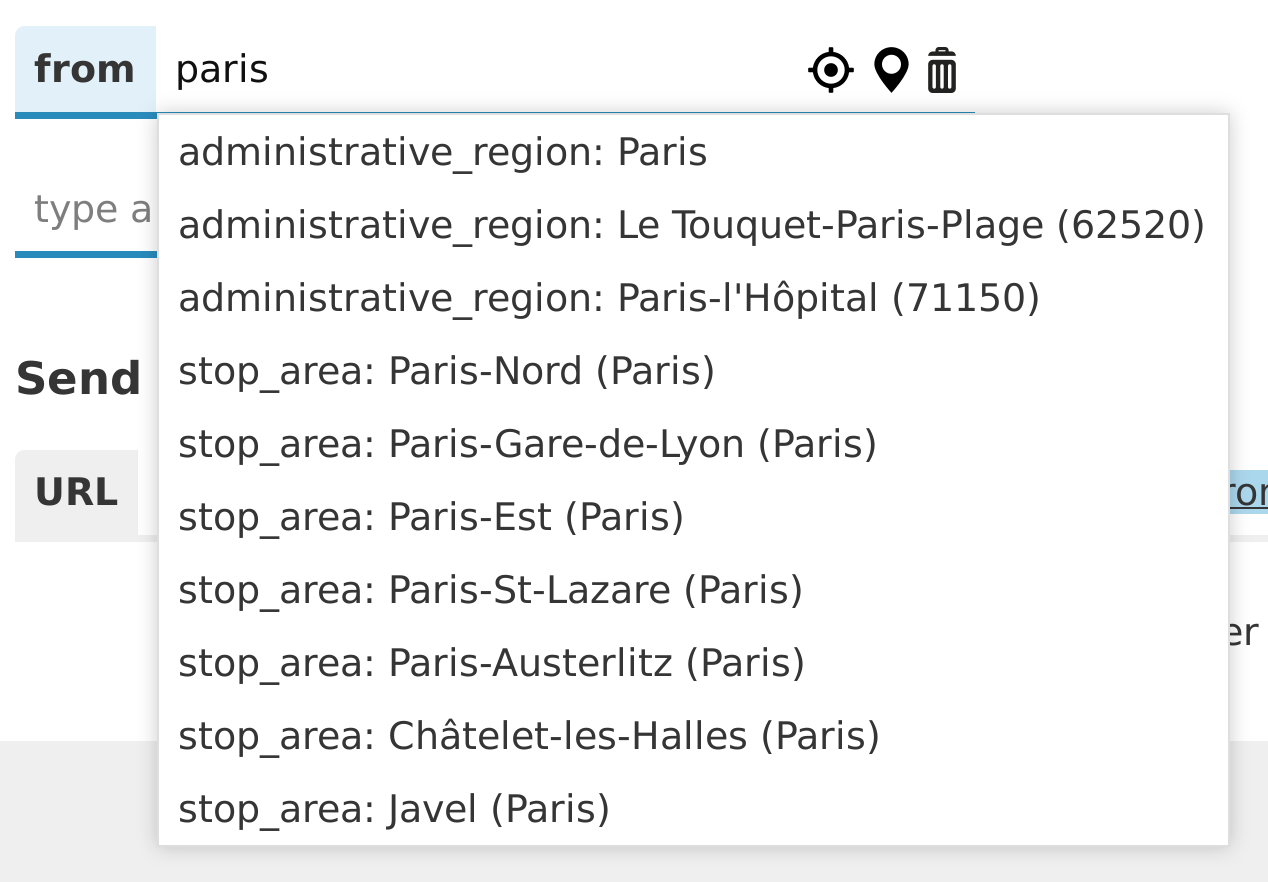
\includegraphics[width=0.7\linewidth]{images/autocomplete-paris}
\end{frame}

\begin{frame}
  \frametitle{Autocompletion tolérante aux fautes}

  \centering
  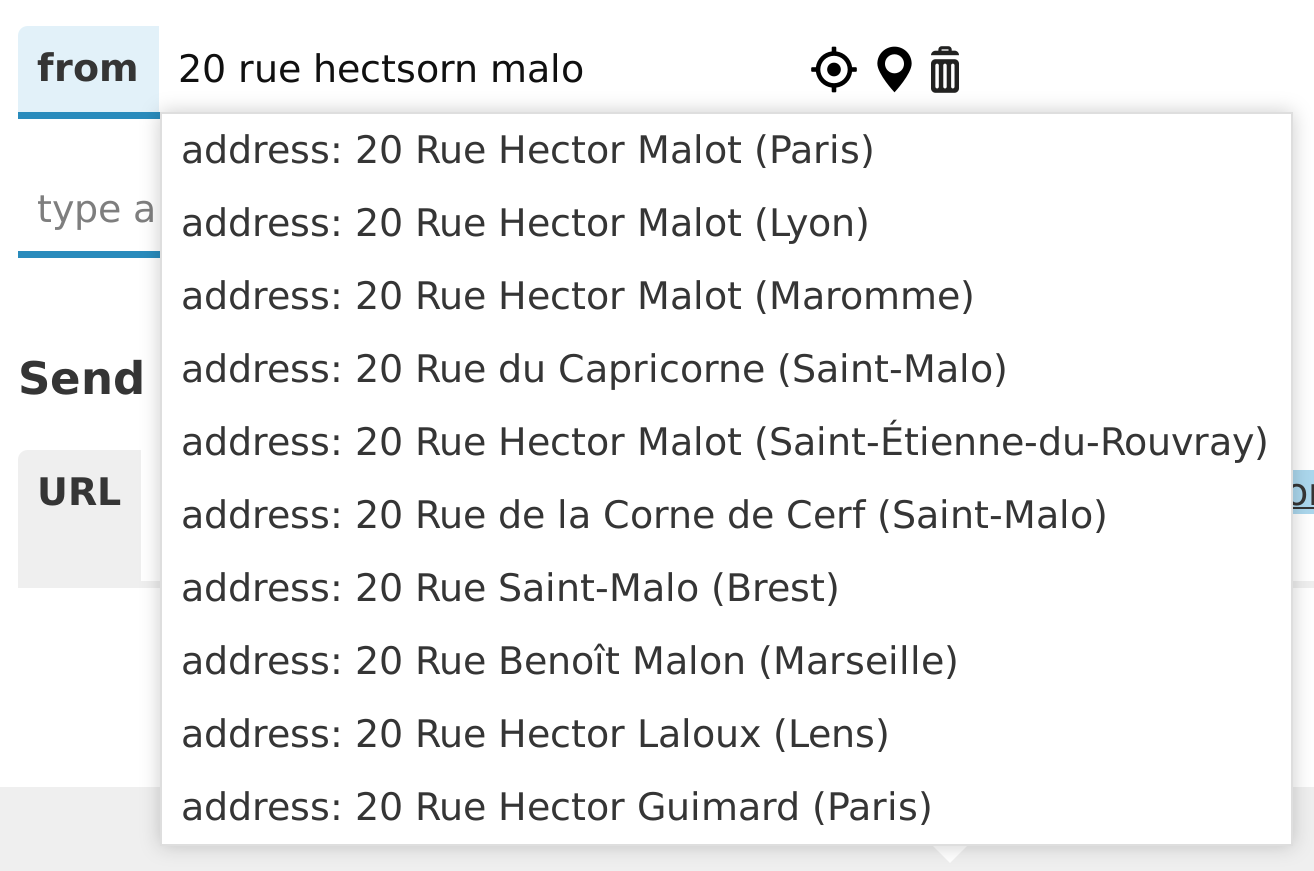
\includegraphics[width=0.7\linewidth]{images/autocomplete-typo}
\end{frame}

\begin{frame}
  \frametitle{Autocompletion par géolocalisation}

  \centering
  \begin{columns}
    \begin{column}{.5\linewidth}
      \begin{block}{\strut Sans coordonnées}
        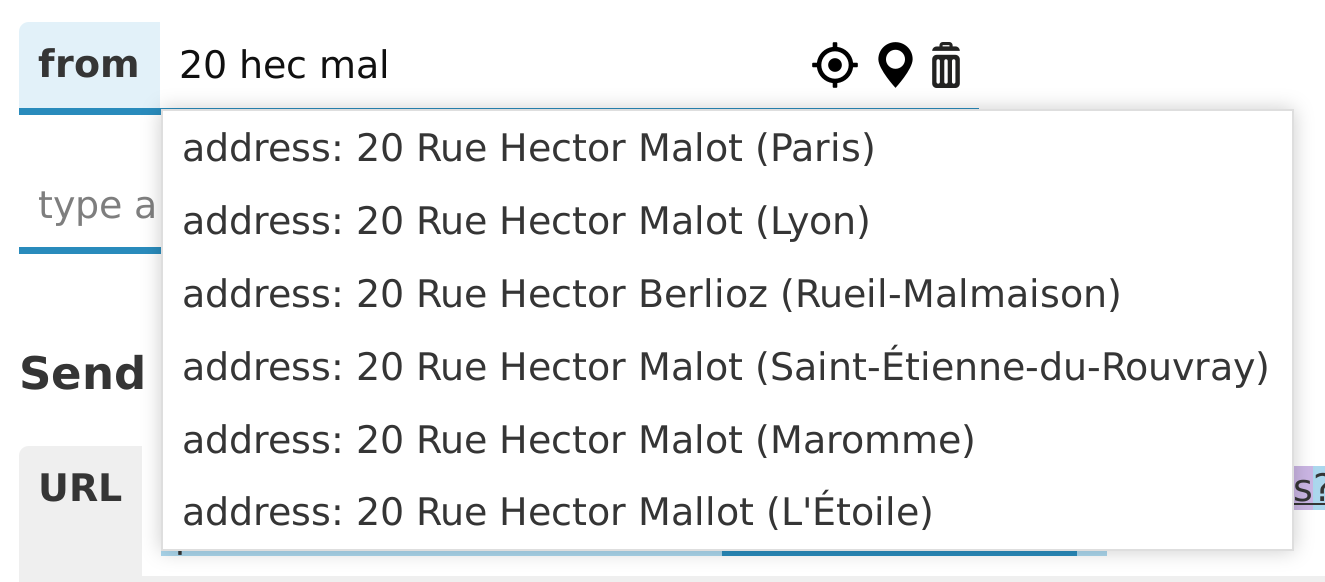
\includegraphics[width=\textwidth]{images/autocomplete-20-hec-mal}
      \end{block}
      \begin{block}{\strut 3 Place de la République (Paris)}
        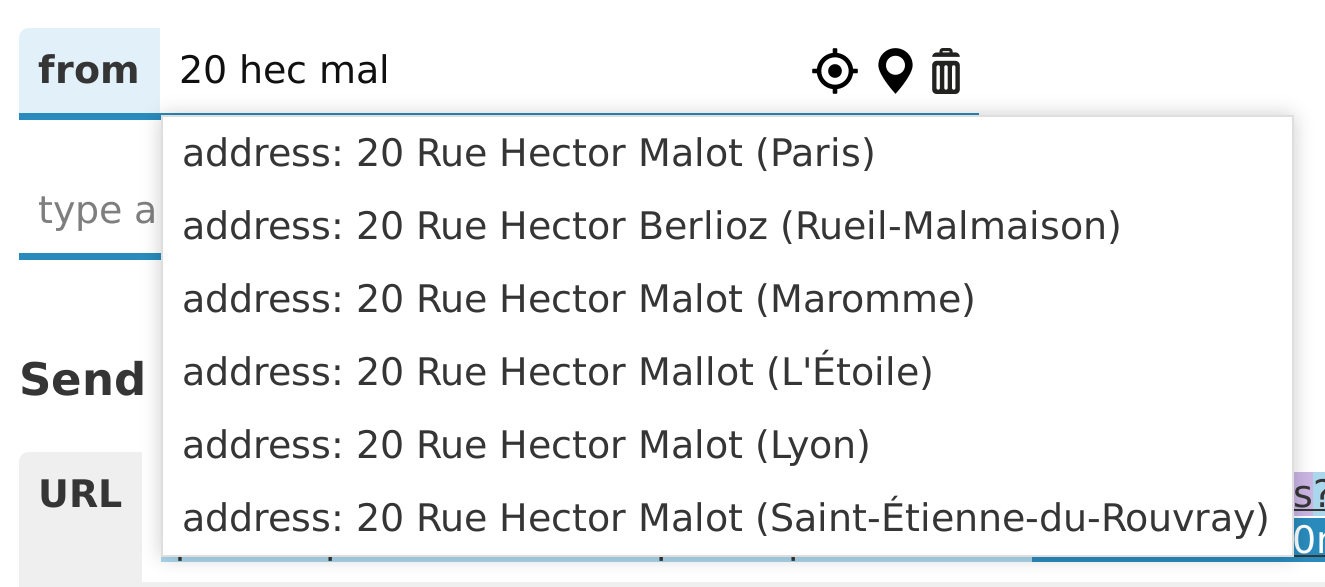
\includegraphics[width=\textwidth]{images/autocomplete-20-hec-mal-paris}
      \end{block}
    \end{column}
    \begin{column}{.5\linewidth}
      \begin{block}{\strut 3 Rue Lebrument (Rouen)}
        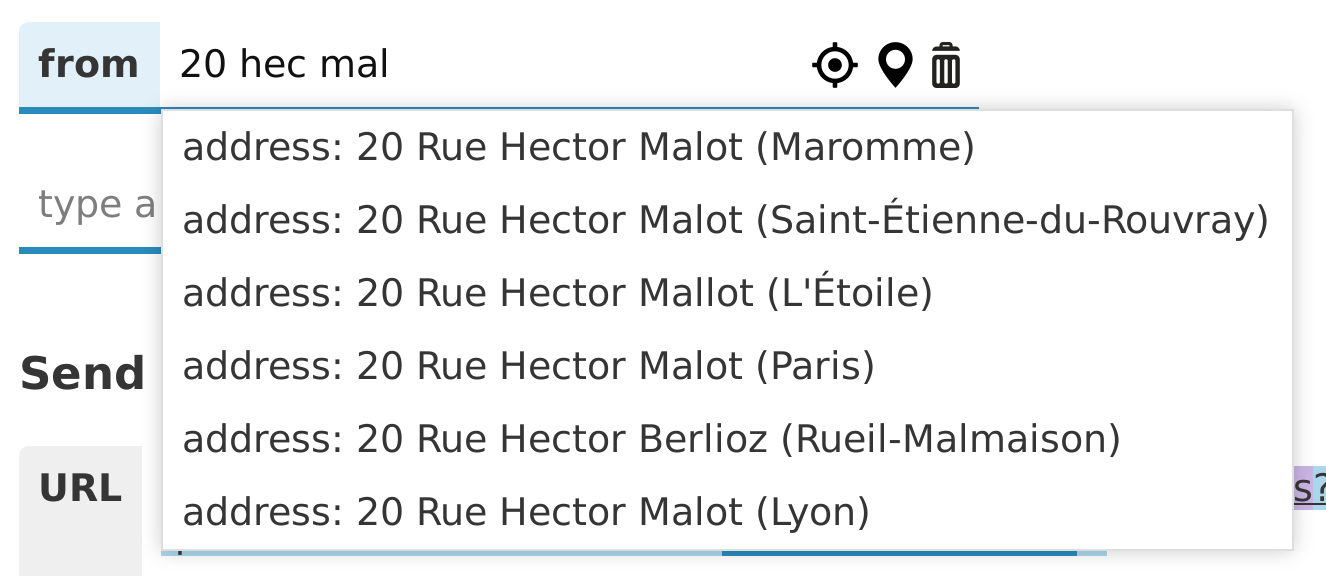
\includegraphics[width=\textwidth]{images/autocomplete-20-hec-mal-rouen}
      \end{block}
      \begin{block}{\strut 2 Rue de la République (Lyon)}
        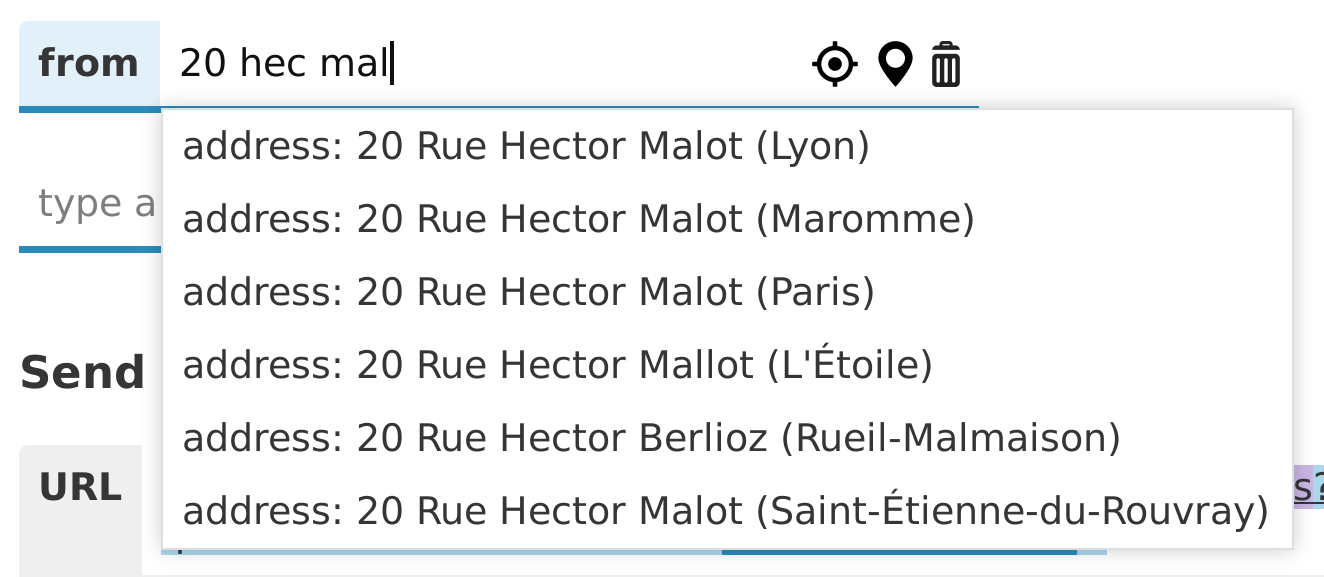
\includegraphics[width=\textwidth]{images/autocomplete-20-hec-mal-lyon}
      \end{block}
    \end{column}
  \end{columns}
\end{frame}

\begin{frame}
  \frametitle{Geolocalisation inversée}

  \centering
  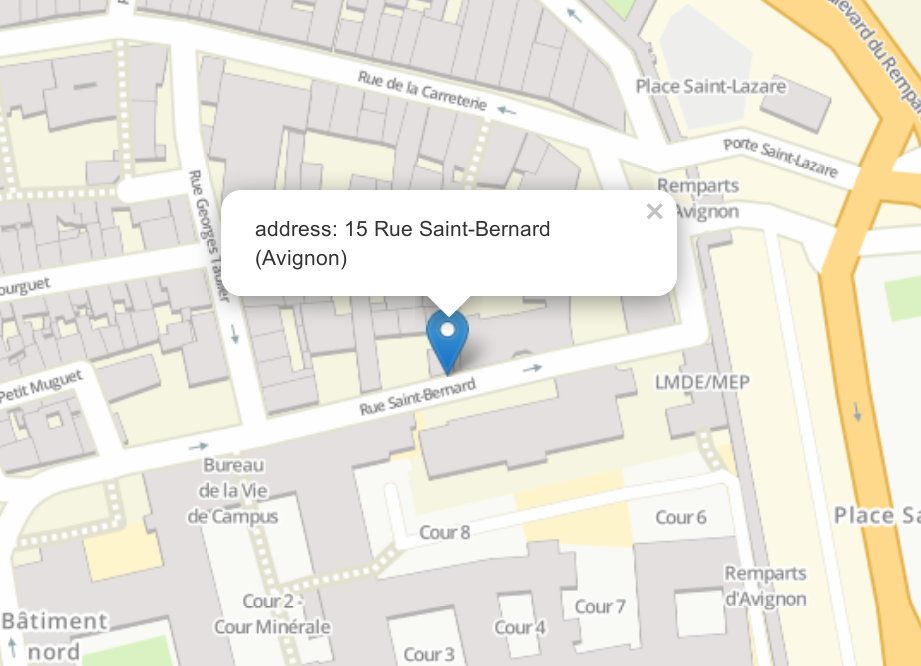
\includegraphics[width=.8\linewidth]{images/reverse-geocoding}
\end{frame}

\section{Technique}

\begin{frame}
  \frametitle{Technique}

  \centering
  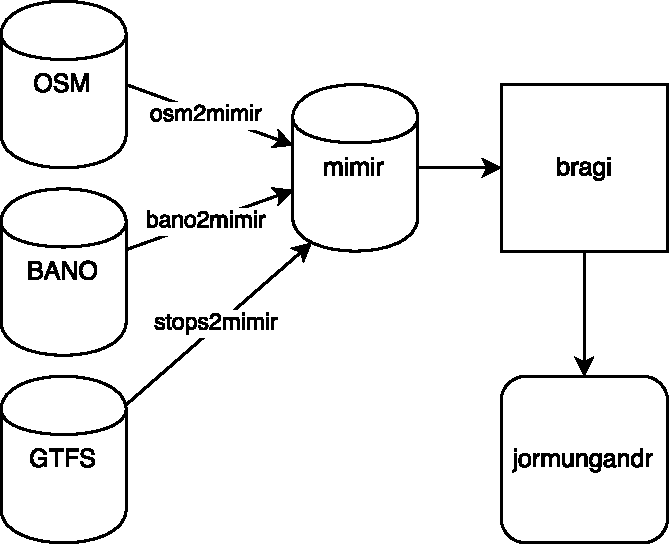
\includegraphics[width=\linewidth]{images/mimirsbrunn}
\end{frame}

\section{Conclusion}

\begin{frame}
  \frametitle{Conclusion}

  Un nouveau système de géocodage:
  \begin{itemize}
  \item opensource: \url{https://github.com/CanalTP/mimirsbrunn}
  \item openservice: \url{https://www.navitia.io/}
  \item qui marche: \href{http://canaltp.github.io/navitia-playground/play.html?request=https\%3A\%2F\%2Fapi.navitia.io\%2Fv1\%2Fplaces\%3Fq\%3D20\%2520hec\%2520mal\%26from\%3D2.364391\%253B48.866436\%26&token=4e5c-bf9d-4fc9-8a60-d47fb98b1b0e}{démo}
  \end{itemize}
\end{frame}

\begin{frame}
  \titlepage
\end{frame}

\end{document}
